\documentclass[a4paper,12pt,final,oneside]{article}

% French characters
\usepackage[frenchb]{babel}
\usepackage[utf8]{inputenc}
% Graphics
\usepackage{graphicx}

\setlength{\parskip}{1ex} %Definit l'espace entre les paragraphes
\pagestyle{empty}

\title{Contes et jeux de rôles}
\author{Rémi Domingues}
\date{\today}

\pagestyle{plain}
\bibliographystyle{plain}

\begin{document}

%Title page
\maketitle

\begin{figure}[h!]
    \centering
    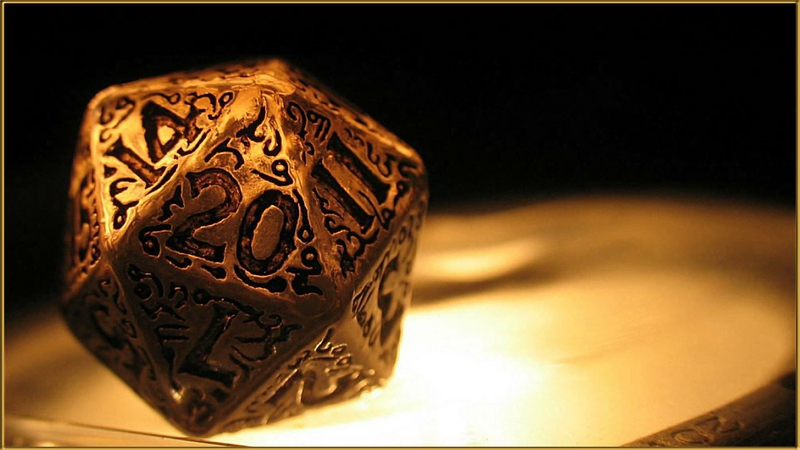
\includegraphics[width=0.80\linewidth]{img/die.jpg}
\end{figure}

\clearpage


%Sommaire
\thispagestyle{empty}
\tableofcontents
\clearpage


\section{Introduction}
\setcounter{page}{1}

Parler des contes en général rapidement, puis du fait qu'ils sont un peu abandonnés. Parler du jeu de rôle, jeu de société oral comportant de fortes similitudes.
Présenter le plan.

\clearpage

jpeg
\section{Le conte, vecteur de transmission d'humanisme en déclin}

« Le premier véritable récit est et demeure le conte », Walter Benjamin, Der Erzähler\cite{benjamin1991gesammelte}

\begin{figure}[h!]
    \centering
    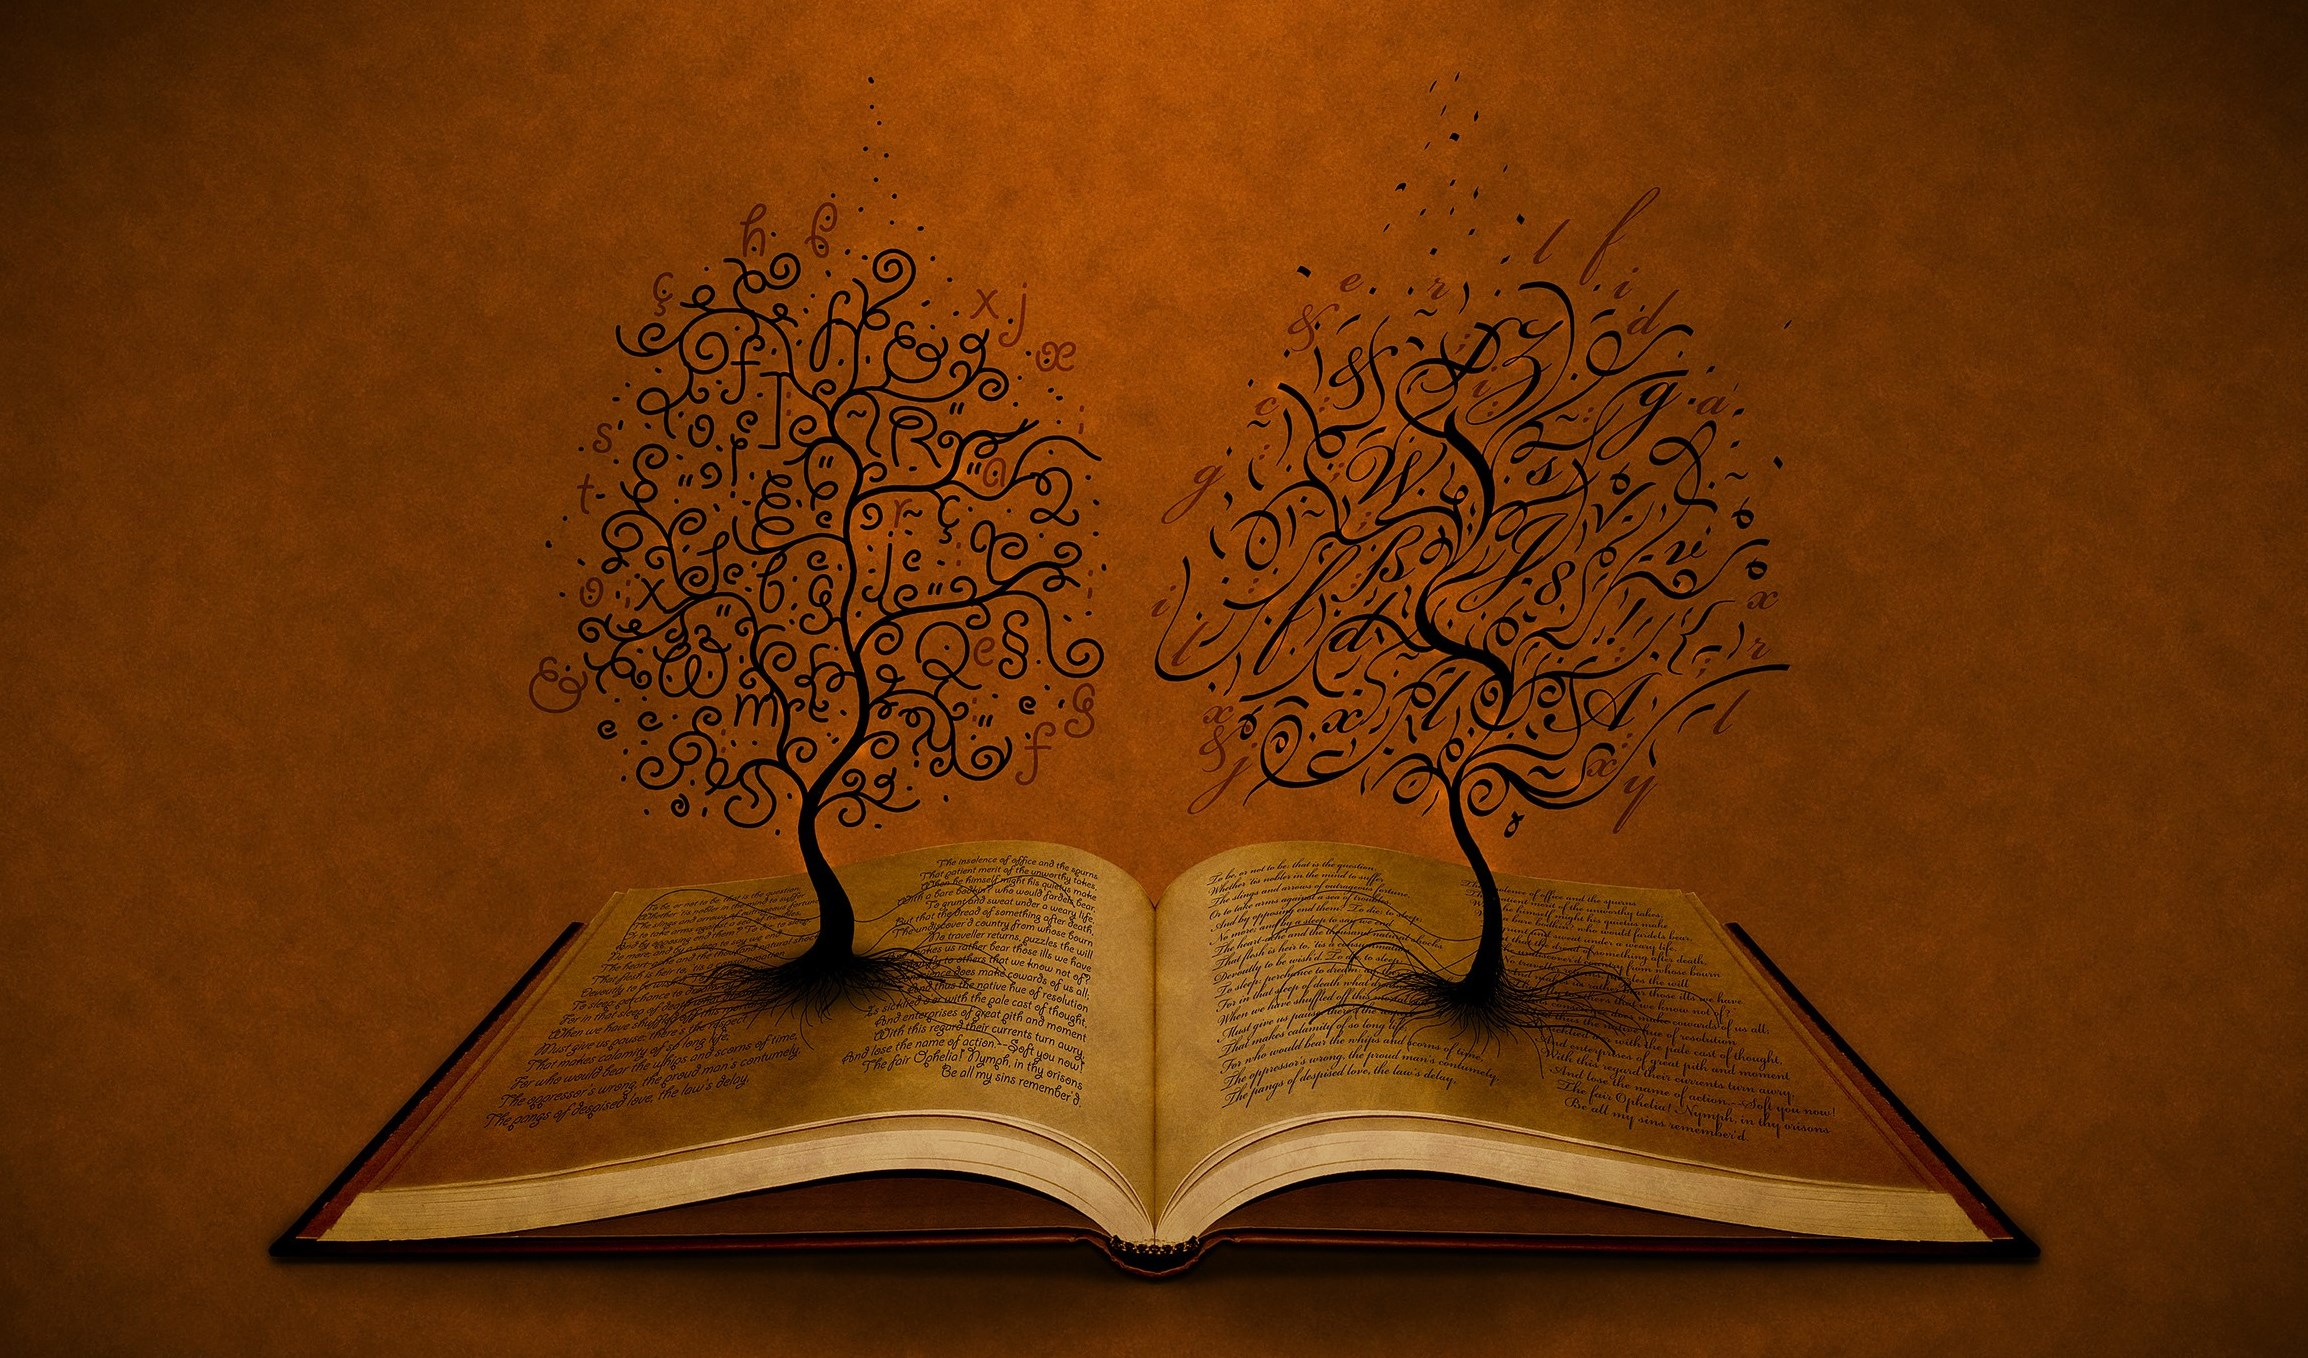
\includegraphics[width=0.80\linewidth]{img/tale_book.jpg}
    \caption{Tale book}
\end{figure}

\subsection{Porteur d'expérience}
Conteur = narrateur\\
Conte opposé au mythe\\
Littérature orale\\

Interprétation Calter Benjamin : \cite{nouss2003conteur}
On parle ici de contes oraux essentiellement
Anciennement et encore aujourd'hui, le conte était un vecteur de perpétuation de l'expérience et de renouvellement de la tradition
La transmission orale via le conte est en perte de vitesse (Walter Benjamin) car elle est essentiellement relative à la transmission d'une expérience, dont l'intérêt porté est en net déclin.\\
Conteurs : sédentaire (perpétuant un lointain temporel constitué de riches expériences passées) / voyageur (rapportant un lointain spatial d'expériences vécues ou entendues en d'autres lieux)\\

L'expérience ici mentionnée peut faire référence à un récit véridique ou bien façonné, porteur d'une morale visant à enrichir l'auditoire du passé, dans le but de guider celui-ci dans les choix futurs qui se poseront à lui.\\
Par ailleurs, le conteur est dans un rapport de proximité avec son auditoire, ce qui permet l'exposé de la distance.\\
Or, cette recherche d'expérience est en perte de vitesse, notamment de par l'information journalistique informant tout un chacun des derniers évènements survenus, prémachés, analysés et expliqués. Au contraire, le conte laisse l'auditoire tirer ses propres conclusions. Le conte délivre en effet un fait nu, exempte de toute explication. La valeur du conte ne réside plus alors dans son intrigue, mais dans la mise en valeur de l'acte de vivre une expérience à proprement parler. C'est donc une conception de l'être humain qui est ainsi véhiculée, celle de vivre des expériences, de traverser des épreuves, et de les surmonter.\\

\begin{figure}[h!]
    \centering
    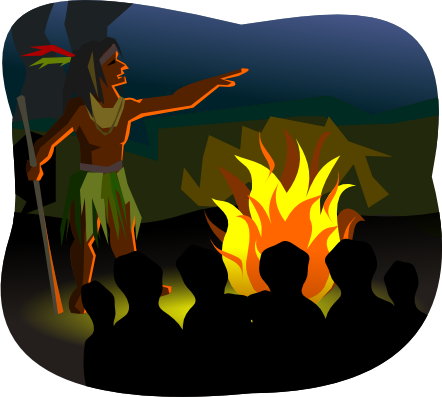
\includegraphics[width=0.80\linewidth]{img/storyteller.png}
    \caption{Storyteller}
\end{figure}

\subsection{L'écoute flottante (à détailler ?)}
Dans l'écoute du conte, le procédé freudien d'attention flottante consistant en l'absence d'attention dirigée ou focalisée, permettrait à l'auditeur de s'oublier lui-même, afin que «les mots qu'il entend[e] s'inscrivent profondément en lui» (ibid), facteur essentiel de l'assimilation et de la mémorisation des contes par l'auditoire via une écoute détendue.\\

\subsection{Le conte et la mort (reformuler)}
«Le parfait récit naît de l'accumulation de ses versions successives». Chaque conteur apose en effet sa marque au récit, transformant celui-ci de par son vécu.\\
L'existence d'un conte réside dans la mémoire de son auditoire, sa survie dans la transmission perpétuée par ses conteurs. Un conte meurt s'il n'est pas transmis.\\
Une cause cause annexe de déclin pourrait résider dans la conception de la mort par l'humain.\\
Selon W. B., le conteur tient de la mort son autorité. En effet, les contes étant faits de vécu, une vie d'expériences fondera donc une sagesse ou un savoir dont la transmission sera d'autant plus riche que la vie en fut emplie :  «La mort est la sanction de tout ce que relate le conteur». À l'heure de sa mort, toute personne devient donc digne d'être écoutée.\\

Le siècle dernier aurait néanmoins bouleversé la conception sociale de la mort dans nos moeurs. Les progrès technologiques et les atrocités commises ont eu pour effet l'acceptation de la conception d'une mort en masse (Hiroshima), pleine de souffrances (camps de déportation), banalisée et quotidienne (médias).\\
La mort étant transformée, l'autorité qu'on en retire en tant que conteur en est également impactée.\\
Les évènements passés ayant bouleversé le rapport mort/vie, ceux-ci ont également impacté la conception que tout un chacun se fait de la survie. La mort d'un être humain conte revêt alors une importance bien moindre, de même que celle d'un conte.


\clearpage


\section{Le jeu de rôle, un renouveau de création populaire}

Le jeu de rôle est un style de jeu à travers lequel une personne incarne un personnage à travers lequel il agît dans un univers fictif. Ces jeux peuvent être réels (on parle alors de jeux de rôle grandeur nature, lorsqu'une personne joue physiquement un personnage de fiction), virtuels (jeux vidéos où le joueur contrôle un avatar) ou «sur table». Nous nous intéresserons ici à cette dernière catégorie, à laquelle se rapportera toute référence aux jeux de rôle dans la suite de cet écrit.

\subsection{Présentation JDR}

«Le principe des jeux de role se rapproche davantage du théâtre improvisé que d'un jeu de société traditionnel» \cite{cristofari2010lecteur}\\
\begin{figure}[h!]
    \centering
    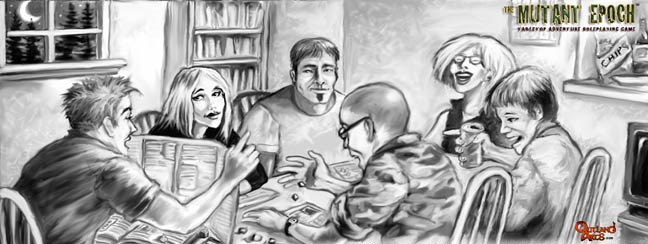
\includegraphics[width=0.80\linewidth]{img/rpg_tabletop1.jpg}
    \caption{Tabletop RPG}
\end{figure}


Jeu de société\\
Un Maître du jeu et entre trois et huit joueurs, chaque joueur interprétant un personnage imaginaire dont les dialogues et actions sont décrites à l'oral. Le maître du jeu, un narrateur, est en charge de choisir ou inventer un monde, une trame aventuresque contée, dans laquelle évolueront les joueurs. Il conte, décrit, fait survenir des évènements à sa convenance, devant également réagit aux actions des joueurs. Il s'agît pour les joueurs de résoudre des énigmes, combattre en équipe (mécanismes de dés afin d'évaluer la réussite d'une action) et vivre une expérience interactive reposant majoritairement sur l'imagination.\\
Une fois l'univers du jeu de rôle défini, les mécaniques du jeu doivent l'être. Il s'agît là de règles permettant d'évaluer la réussite des actions entreprises par les personnages joueurs et non joueurs, faisant souvent appels à des sets de dés dont le nombre de face varie usuellement de 4 à 20, l'interprétation des résultats dépendant en outre des caractéristiques des personnages concernées.\\
Un jeu de rôle n'a pour public que son maître du jeu et ses joueurs.\\
Le but d'une partie de jeu de rôle n'est pas tant de remporter la partie, le scénario de celle-ci pouvant être étendue avec pour seule limite la créativité du maître du jeu, mais plutôt de prendre plaisir à l'expérience imaginaire et sociale vécue. La partie, le plus souvent étalée sur plusieurs semaines, voire mois, prendra alors fin lorsque le maître du jeu estimera le monde suffisamment exploré, le scénario principal accompli ou par simple manque de temps. Il n'y a donc ni gagnant, ni perdant, le but étant la coopération des joueurs afin de vivre une aventure.\\

Les univers dont sont inspirés les mondes et scénarios ont souvent une origine littéraire (Call of Cthulhu, Lovecraft => ref, Le seigneur des anneaux, Tolkien) ou cinématographique (Star Wars).\\
La fidélité à l'oeuvre est alors libre au maître du jeu. On peut ainsi observer des fictions en accord irréprochable avec l'oeuvre dont elle sont issues, comme d'autres s'en inspirant vaguement, voire inventant un monde depuis ses fondements. Il en est de même pour le respect aux règles des jeux de rôles.\\
De nombreux livres de règles ont en effet été édités, chacun véhiculant avec lui la description étendue d'un monde, des races (humain, nain, elfe...) et classes (catégorie, telle magicien, prêtre, épéiste, chevalier...) de personnages, mais également des règles de jeu et un set de scénarios prédéfinis. Le respect de ces ouvrages est également laissé libre à chacun.\\

\begin{figure}[h!]
    \centering
    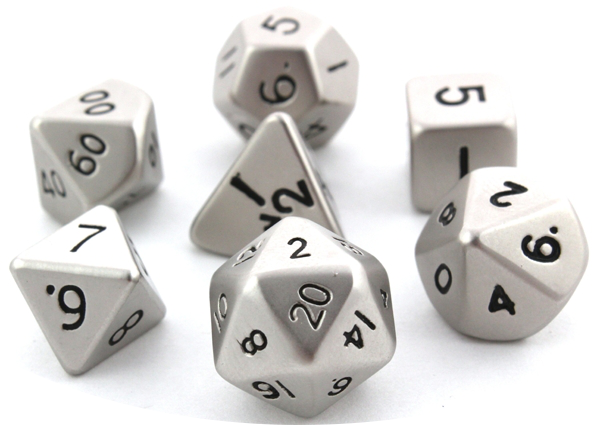
\includegraphics[width=0.80\linewidth]{img/dice_set.png}
    \caption{Dice set}
\end{figure}

\subsection{L'attrait des joueurs}
L'attrait des joueurs pour les jeux de rôle proviet essentiellement de l'identification des joueurs au personnage que ceux-ci jouent, souvent plus importante que l'histoire vécue, pouvant entraîner une forte addiction, du même acabit que celle pouvant être constatée sur des jeux vidéos.

Le but du jeu de rôle est aussi d'étendre l'intrigue d'une oeuvre de fiction.

L'attrait des joueurs proviendrait selon Olivier Caïra\cite{caira2007jeux} de la multitude et de la complexité des compétences à mettre en oeuvre afin de pratiquer ce mode de jeu. Il s'agit en effet d'une cohabitation entre un maître du jeu et ses joueurs, ceux-ci devant effectuer une répartition des rôles au sein de leur équipe dans l'objectif d'augmenter leur efficacité à répondre aux évènements rencontrés par une complémentarité adéquate. Par ailleurs, la communication dont font preuve les joueurs se doit d'évoluer constamment, d'une part de par le niveau du registre de langue utilisé, mais également vis-à-vis de leur degré d'immersion dans le jeu (descriptions, commentaires hors du jeu, dialogues, précisions). Les joueurs doivent enfin faire preuve compétences variées (cohésion de groupe, éloquence, stratégie...) qui peuvent ici être perfectionnées.

\subsection{Psychanalyse}
Le jeu de role est en outre utilisé dans le domaine de la psychanalyse, considéré comme une aire d'expérience où les réactions de l'individu vis-à-vis de son environnement peuvent être analysées.

Étant bien souvent moins proche de la réalité que les contes, on peut y rencontrer davantage de stéréotypes, les joueurs choisissant souvent de s'idéaliser à travers le personnage joué afin d'obtenir dans ce monde imaginaire une place que ceux-ci ne parviennent pas à atteindre dans le monde réel.\\
Les joueurs peuvent aussi interpréter leur opposé (une personnalité extravertie pour un joueur timide, un fanatique religieux pour un athée). Ces jeux de rôles peuvent également être le lieu de réalisation de fantasmes et évènements socialement inacceptable dans le monde réel.



\clearpage

\section{Le jeu de rôle, un conte interactif}

«L'art de raconter des histoires est toujours l'art de reprendre celles que l'on a entendues»\\

\begin{figure}[h!]
    \centering
    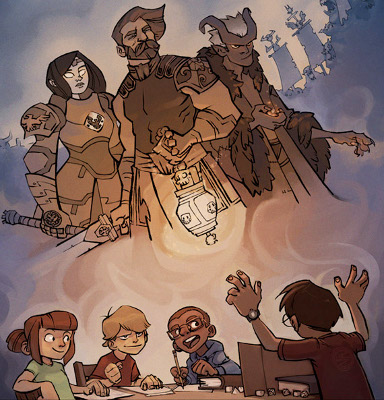
\includegraphics[width=0.80\linewidth]{img/rpg_tabletop2.jpg}
    \caption{Tabletop RPG}
\end{figure}

Différence entre conte et jeu de role : \\
- Personnages joueurs interagissant dans une histoire que le maître du jeu déroule pour eux, celui-ci s'adaptant à ses joueurs\\
- Univers souvent imaginaire\\
- Rarement porteur de morales, mais plutôt d'aventures\\


Similitudes :\\
- Aspect social\\
- Histoire racontée à l'oral\\
- Conteur et Maître du jeu : transporter son auditoire dans l'imaginaire\\
- Rôle essentiel de l'ambiance instaurée afin de maximiser l'immersion, et éventuellement de faire passer un message, une morale\\
- Pratique des jeux de rôle associables aux récits chevaleresques contés par les troubadours\\
- Le maître du jeu adapte son scénario aux réactions de ses joueurs. Le conteur en fait de même, en fonction de celles de son public. Le conte s'étaye par ailleurs au fil des représentations, et l'analyse des réactions du public est la clé de l'amélioration d'un conte\\

Rôle psychanalytique :\\
- L'immersion dans l'histoire permet de libérer des instincts primitifs et l'analyse des auditeurs\\
- Stimule l'imagination, dévoile des émotions et permet de mieux connaître et découvrir nos difficultés pour lesquelles nous étayons peu à peu inconsciemment des solutions\\

\clearpage



\section{Conclusion}
TODO : lettre ae\\
Le jeu de rôle est donc une sorte de conte interactif
TODO : étayer en relisant le pph (son aspect novateur, ce qu'il apporte en plus du conte, pourquoi c'est chouette d'être roliste...)
Conte = vecteur d'expérience, dont le cours est en baisse
Jeux de rôle = vivre une expérience !
\clearpage

\section{Bibliographie}
\def\section*#1{} % Supprime le titre "References" et l'espace qui lui etait alloue
\bibliography{references}

Gilles Brougère
Brian Sutton-Smith
Jacques Henriot

\end{document}